%!TEX root = /Users/tcya/Dropbox/XunmoYang/PhDthesis/thesis.tex
\chapter{Introduction}\footnotetext{Part of this chapter has been published in Xunmo Yang and E. R. Bittner, The Journal of Physical Chemistry A\textbf{118}, 5196 (2014)}
\section{Introduction}

Energy and electronic transport plays a central role in a
wide range of  chemical  and biological systems.
It is the fundamental mechanism for transporting the  energy  of an
absorbed photon to a reaction center in light harvesting systems
and for initiating a wide range of photo-induced  chemical processes,
including vision, DNA mutation, and pigmentation.
The seminal model for calculating electron transfer rates was developed by
Marcus in the 1950's\cite{marcus1956theory,marcus1965theory,marcus1993electron}.
\begin{equation}
k_{Marcus}=\frac{2\pi}{\hbar}|V_{ab}|^{2}\frac{1}{\sqrt{4\text{\ensuremath{\pi}}k_{B}T\lambda}}e^{-(\lambda+ \Delta\epsilon)^{2}/4\text{\ensuremath{\lambda}}k_{B}T}.\label{eq:marcus}
\end{equation}
where $\lambda$ is  energy required to reorganize the environment
following the transfer of an electron from donor to acceptor.
and $\Delta \epsilon$ is the driving force for the reaction, as illustrated in Fig.~\ref{marcus}. If we assume that the nuclear motions about the equilibrium configurations of the
donor and acceptor species is harmonic,  the chemical reactions resulting from
energy or charge transfer events can be understood in terms of intersecting
diabatic potentials as sketched.    The upper and lower
curves are the adiabatic potential energy surfaces describing the nuclear dynamics
resulting from an energy or charge transfer event, taking the geometry of the donor
state as the origin.

\begin{figure}[h]
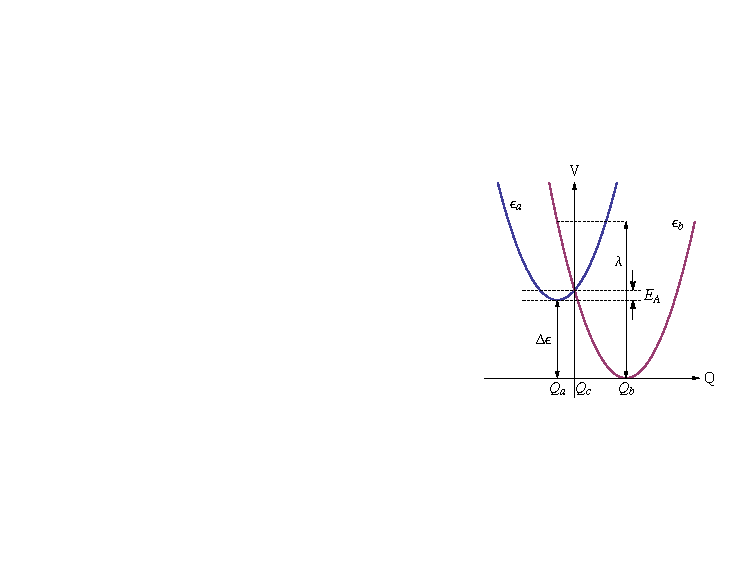
\includegraphics[width=0.5\columnwidth]{Chapters/chap2/Figure1}
\caption{Sketch of Marcus parabolas for a model energy or charge transfer system.
Labeled are the key parameters used to compute the Marcus rate constant (Eq. \ref{eq:marcus}).
Energies are given in eV and the collective nuclear displacement  is dimensionless.
}
\label{marcus}
\end{figure}

%For reactions carried out in open systems,  the Marcus parabolas represent
%free energy surfaces with driving force $\Delta G$.
As the transfer occurs by crossing an energy barrier,
the transfer rate can be expected to be in the Arrhenius form
\begin{eqnarray}
k\propto e^{-E_{A}/k_{B}T},
\end{eqnarray}
with $E_{A}$ as the activation energy.
 Using $E_{A}={(\lambda+\Delta \epsilon)^{2}}/{4\lambda}$
 we can relate the activation energy to both the reorganization energy and driving force, $-\Delta \epsilon$.
One of the most profound predictions of the theory is that  as the driving force increases,
the transfer rate reaches a maximum and further increases in the driving force
lead to lower reaction rates, termed the inverted regime. The inverted region is unequivocally substantiated by Miller {\em et al.} \cite{miller1984intramolecular} in a series experiments of intramolecular transfer. Part of their work is used as the experimental benchmark of our model in Chapter \ref{chap:chapt2} and \ref{chap:chapt3}.




A number of years ago,  our group developed a time-convolutionless  master equation approach for computing
state-to-state rates in which the coupling between  states depends upon the
nuclear coordinates\cite{pereverzev2006time}. This approach incorporates a fully quantum
mechanical treatment of both the nuclear and electronic degrees of freedom and recovers the
well-known Marcus expression in the semiclassical limit.  The model is parameterized by the
vibrational normal mode frequencies, and the electronic energies and energy derivatives
at a reference configuration.  The approach has been used by our group to compute state-to-state
transition rates in semi-empirical models for organic semiconducting light-emitting diode and photovoltaics
\cite{tamura2008phonon,tamura2007exciton,bittner2014noise,singh2009fluorescence}.
Our work here represents the first time this approach has been used within the context of a fully {\em ab initio} quantum
chemical model.   As such, this present work provides an important benchmark of the approach since all parameters will be determined
using state-of-the-art quantum chemical methods
and results compared to both theoretical and experimental
rates.

% Central to the work presented here consists of two parts. One is the use of a diabatization scheme for determining
% donor and acceptor states in a molecular unit. The other is a projection scheme which enables us to analyze the contribution of vibrations in reactions. Similar decomposition schemes have been presented by Burghardt
%  \cite{cederbaum2005short,gindensperger2006shortI,gindensperger2006shortII,cederbaum2005short}
%  and the approach used here builds upon the method given in Ref.~\cite{pereverzev2009energy}. In Chapter \ref{chap:chapt2} we benchmark the approach
% by computing the  triplet energy transfer rates for a series of donor-bridge-acceptor molecules
% originally studied by Closs\cite{miller1984intramolecular}.  The triplet energy transfer rates computed using our approach
% compare well against both the experimental rates and with
% more recent theoretical rates presented by Subotnik {\em et al.}
% \cite{subotnik2008constructing,subotnik2009initial,subotnik2010predicting}.
% Then we use the projection operator scheme
% to parses out specific internal nuclear motions that accompany
% the electronic transition.
%  By analyzing the electron-phonon couplings, we can
% discern a reduced set of motions that are responsible for coupling between the donor and
% acceptor states.



\section{Theoretical Approach}\label{section:theory}
Below we give a detailed description of our methods.

\subsection{Model Hamiltonian}
We consider a generic model for $n$ electronic states coupled linearly
to a phonon bath.  Taking the electronic ground state of the system as a reference
and assuming that the electronic states are coupled linearly to a common set of
 modes, we arrive at a generic form for the Hamiltonian, here written for two coupled electronic states:
 \begin{eqnarray}
H=\left(\begin{array}{cc}
\epsilon_{1} & 0\\
0 & \epsilon_{2}
\end{array}\right)+\left(\begin{array}{cc}
{\mathbf g}_{11}&{\mathbf g}_{12} \\
{\mathbf g}_{21} &{\mathbf g}_{22}
\end{array}\right)\cdot{\mathbf q} +\frac{{\mathbf p}^{2}}{2}+\frac{1}{2}\mathbf{q}^{T}\cdot\mathbf\Omega\cdot\mathbf{q}.
\nonumber \\
\label{ham1}
\end{eqnarray}
Here, the first term contains the electronic energies, $\epsilon_{1}$ and $\epsilon_{2}$ computed at a
reference geometry--typically that of the donor or acceptor state.   The second term represents the
linearized coupling between the electronic and nuclear degrees of freedom given in terms of the mass-weighted
normal coordinates $\mathbf q$. The equation assumes the potentials for the excited states are parabolic. This is usually valid in the reaction region, as we will show in next several chapters.  The diagonal terms
give the adiabatic displacement forces between the reference geometry and the two states.  If we choose one of the
states as the reference state, then either $\mathbf g_{11}$ or $\mathbf g_{22}$ will vanish.
The remaining two terms correspond to the harmonic motions of the nuclear normal modes, given here in mass-weighted normal coordinates.
In the normal mode basis, the Hessian matrix, $\mathbf \Omega$,  is diagonal with elements corresponding to the normal mode frequencies, $\omega_{j}^{2}$.


We now separate Eq.~\ref{ham1} into diagonal and
off-diagonal terms
\begin{eqnarray}
\hat  H = \hat H_{o} + \hat V
\end{eqnarray}
and perform a polaron transform
using the unitary transformation~\cite{grover1970exciton,rice1994excitons,pereverzev2006time}.
\begin{eqnarray}
U&=&e^{-\sum_{ni}\!\!\frac{g_{nni}}{\hbar\omega_i}|n\rangle \langle
n|(a^{\dagger}_i-a_i)}
 \nonumber \\
&=&
\sum_{n}|n\rangle \langle n|e^{-\sum_{i}\!\!\frac{g_{nni}}{\hbar\omega_i}(a^{\dagger}_i-a_i)}
\label{unitary}
\end{eqnarray}
under which the transformed Hamiltonian is written in terms of the
diagonal elements
\begin{eqnarray} \tilde H_0=U^{-1}H_0U
=\sum_n\tilde\epsilon_n |n\rangle \langle
n|+\sum_i\hbar\omega_ia^{\dagger}_ia_i,
 \end{eqnarray}
with  the renormalized electronic energies,
\begin{eqnarray}
\tilde\epsilon_n=\epsilon_n-\sum_{i}\frac{g_{nni}^2}{\hbar\omega_i},
\end{eqnarray}
and off-diagonal terms,
\begin{eqnarray} \hat V_{nm}=\sum_{i}g_{nmi}\left(a^{\dagger}_i+
a_i-\frac{2g_{nni}}{\hbar\omega_i}\right)e^{\sum_{j}\frac{(g_{nnj}-g_{mmj})}{\hbar\omega_j}(a^{\dagger}_j-a_j)}.
\label{opm}
\end{eqnarray}
In the transformed (or dressed) picture the electronic transition from state
$|n\rangle$ to $|m\rangle$ is accompanied by the excitations of all the
normal modes. Following the conventional notations in this field, we refer to all harmonic nuclear motions as phonons. Transforming to the interaction representation
and performing a trace over the phonons gives the spectral density in
terms of the autocorrelation of the electron-phonon coupling
operators.
\begin{eqnarray}
S_{nm}(\tilde\omega) = \int_{-\infty}^{\infty} \! \mathrm{d}t e^{-i\tilde \omega t}\langle \hat V_{nm}(t) \hat V_{mn}(0)\rangle.\label{spec-dens}
\end{eqnarray}
Here, $\hat V_{nm}(t)$ is the electron-phonon coupling term in the Heisenberg representation and
$\langle \cdots \rangle$ denotes a thermal average over the
vibrational degrees of freedom.
The derivation and explicit form for the kernel in Eq.~\ref{spec-dens}  is quite lengthy and is given in
Ref.~\cite{pereverzev2006time}.

\subsection{Non-Markovian Master Equation and Golden-Rule Rates}

In Ref.~\cite{pereverzev2006time}, Pereverzev and Bittner derived
a non-Markovian, time-convolutionless form of the Pauli master
equation (TCLME)  for general system described by Eq.~\ref{ham1}.
\begin{eqnarray}
\frac{dP_{n}}{dt} = \sum_{m \ne n} W_{nm}(t)P_{m}(t) - \sum_{m \ne n} W_{mn}(t)P_{n}(t)
\end{eqnarray}
where the time-dependent rates are given by
\begin{eqnarray}
W_{nm}(\tau)=2{\rm Re}\int_{0}^{\tau} \! \mathrm{d}t\left\langle \hat V_{nm}(0)\hat V_{mn}\left(t\right)\right\rangle e^{-i\tilde\omega_{nm}t}.
\label{rate-expression}
\end{eqnarray}
In the limit that $\tau\to\infty$, Eq.~\ref{rate-expression} gives the Fermi's Golden Rule expression for the
transition rate,
\begin{eqnarray}
k_{nm}=2{\rm Re}\int_{0}^{\infty} \! \mathrm{d}t\left\langle \hat V_{nm}(0)\hat V_{mn}\left(t\right)\right\rangle e^{-i\tilde\omega_{nm}t}.
\label{gr-expression}
\end{eqnarray}

At this point it is useful to connect the various terms in the phonon-dressed Hamiltonian
with specific physical parameters.
First, the reorganization energy is given by
%The terms involving $$
%are related to the reorganized energy difference between the two states.
%$$
%\lambda_{nm} =\sum_{j}((g_{nnj}-g_{mmj})/\omega_j)^{2} = \sum_{j}\hbar \omega_{j}S_{j}
%$$
\begin{eqnarray}
\lambda_{nm}=\sum_{j}\frac{\left(g_{nnj}-g_{mmj}\right)^{2}}{\omega_{j}} = \sum_{j}\hbar \omega_{j}S_{j}
\end{eqnarray}
where  the $\{S_{j}\}$  are  the Huang-Rhys factors for each phonon mode.
These are related to the Franck-Condon factor
describing the overlap between the $v_j=1$ vibronic state in one electronic state
with the $v_j=0$ vibronic state in the other.
Likewise, the energy difference between the renormalized energy gaps is related to the
driving force of the state-to-state transition,
\begin{eqnarray}
\Delta E_{nm} = \tilde \epsilon_n-\tilde \epsilon_m.
\end{eqnarray}


We first developed the approach about 10 years ago. However, the difficulty in using this approach is that
it requires both diagonal (${\mathbf g}_{nn}$) and off-diagonal  (${\mathbf g}_{nm}$) derivative couplings between
adiabatic states.    In the following section, we discuss how we have used the Edmiston-Ruedenberg (ER) localization scheme \cite{edmiston1963localized} to estimate the couplings.   We also present how one can construct a reduced set of harmonic modes that
fully capture the electron/nuclear coupling.




\subsection{Adiabatic and Diabatic Representations}
There are two common ways to represent the Hamiltonian, adiabatic and diabatic representations, as sketched in Fig. \ref{adiaDiab}. The way we represent the Hamiltonian in Eq. \ref{ham1} is adiabatic representation, where states are the eigenstates of molecule, and hence can be directly calculated in {\em ab initio} quantum chemistry software. However, the off-diagonal couplings in adiabatic representations ($g_{ij}$ in Eq. \ref{ham1}) are derivative couplings, which are difficult to compute. Even worse, the  couplings change radically near avoided crossing. A workaround is switching to diabatic representation, where the Hamiltonian is written as
\begin{eqnarray}
H_{dia}=U^{T}H_{adia}U=\left(\begin{array}{cc}
\epsilon_{a}(\mathbf{R})\mathrm{+T'_{n}}(\mathbf{R})_{11} & V_{ab}\\
V_{ab} & \epsilon_{b}(\mathbf{R})\mathrm{+T'_{n}}(\mathbf{R})_{22}
\end{array}\right).
\end{eqnarray}

The diabatic representation has several advantages. First, sharp derivative couplings in adiabatic representations are transformed to smoother static diabatic couplings, $V_{ab}$. Second, potential energy surfaces are  smoothened and avoided crossing is eliminated.


\begin{figure}[!t]
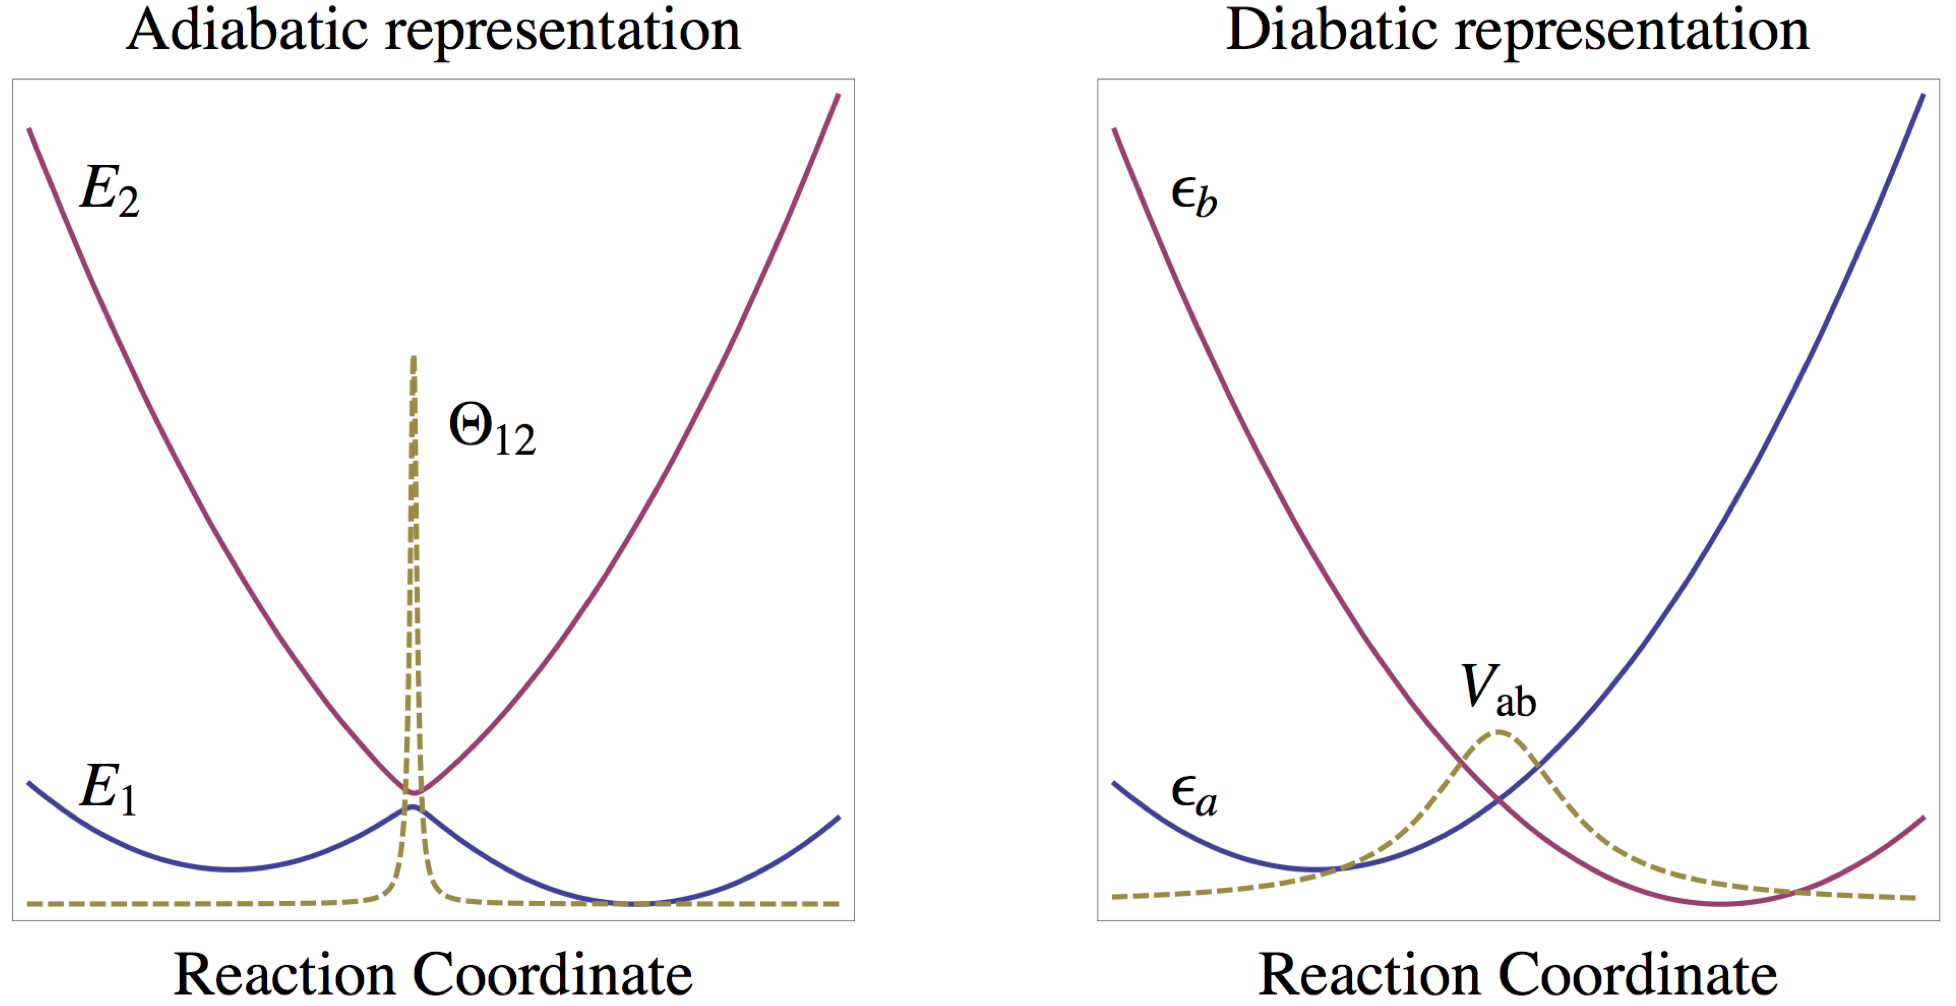
\includegraphics[width=0.95\columnwidth]{Chapters/chap2/adia_vs_diabatic.png}
\caption{Sketch of adiabatic and diabatic representations for two-state system. Compared to adiabatic representation, diabatic representation has smoother energy surfaces and couplings.
}
\label{adiaDiab}
\end{figure}

The problem now is how to obtain the transformation matrix
\begin{eqnarray}
U = \left(\begin{array}{cc}
\cos\theta & \sin\theta\\
-\sin\theta & \cos\theta
\end{array}\right).
\end{eqnarray}
There are many methods available \cite{domcke2004conical}. Here we introduce the Edmiston-Ruedenberg diabatization approach.


\subsection{Edmiston-Ruedenberg Diabatization}\label{sec:ER}
A straightforward way to construct diabatic states is to eliminate derivative coupling mathematically, namely, to solve
\begin{eqnarray}
\left\langle \phi_{i}(\mathbf{r};\mathbf{R})|\nabla_{\mathbf{R}}|\phi_{j}(\mathbf{r};\mathbf{R})\right\rangle = 0.
\end{eqnarray}
However, it is computationally very expensive, and exact solution do not usually exist \cite{mead1982conditions}.

Another category of diabatization methods is based on physical intuition, with ER diabatization being one of them. The ER diabatization is based on the idea that good diabatic states are supposed to be localized, so the approach defines the diabatic states by maximizing the total electron repulsion
\begin{eqnarray}
f_{ER}=\sum_{k}^{N_{states}}\iint dr_{1}dr_{2}\frac{\left\langle \phi_{k}|\hat{\rho}\left(r_{1}\right)|\phi_{k}\right\rangle \left\langle \phi_{k}|\hat{\rho}\left(r_{2}\right)|\phi_{k}\right\rangle }{\left\Vert r_{1}-r_{2}\right\Vert }.
\end{eqnarray}

\subsection{Parameterization From Quantum Chemistry}

 In order to obtain the final form of our target Hamiltonian, we assume the diabatic  potentials
are a good approximation to the actual adiabatic potentials.

When the adiabatic (and diabatic) energy minima
are far enough away from the crossing points and the mixing angles between the diabatic  and adiabatic
states is small, we can
use the gradients of the adiabatic potentials to approximate the diabatic potentials.
Thus, if we perform calculations at the
optimized geometry of the final acceptor state  ({\em i.~e.} about $Q_{2}$  in Fig.~\ref{marcus}),
we can write the Hamiltonian as
\begin{eqnarray}
H_{dia,e}=\left(\begin{array}{cc}
\epsilon_{1} & V_{12}\\
V_{21} & \epsilon_{2}
\end{array}\right)+\left(\begin{array}{cc}
0 & 0\\
0 & 1
\end{array}\right) {\mathbf g}_{22}\cdot{\mathbf q}+H_{osc},
\end{eqnarray}
where $H_{osc}$ is the harmonic oscillator Hamiltonian for the vibrational normal modes.
The linear assumption amounts  to performing a series expansion of the
full, multi-dimensional coupling term and keeping only the lowest order terms.
Systematic improvement can be made by including higher-order (e.g.  quadratic) off-diagonal couplings.
However, this would involve a substantial increase in the complexity of the theory.
The linear assumption is reasonable so long as  the mixing angle is small,
as verified by the benchmark calculations presented below.

We obtain the diabatic couplings $V_{12}$
and the mixing angle $\theta$  via ER localization and transform the electronic Hamiltonian
from the adiabatic basis to the diabatic basis {\em viz.}
\begin{equation}
H_{dia}=\left(\begin{array}{cc}
\cos\theta & -\sin\theta\\
\sin\theta & \cos\theta
\end{array}\right)\left(\begin{array}{cc}
\epsilon_{1}  & 0 \\
0  & \epsilon_{2}
\end{array}\right)\left(\begin{array}{cc}
\cos\theta & \sin\theta\\
-\sin\theta & \cos\theta
\end{array}\right).\label{eq:boys}
\end{equation}
The diabatic coupling is then given by
\begin{eqnarray}
V_{ab}=\frac{1}{2}\sin2\theta\left(\epsilon_{2}-\epsilon_{1}\right).\label{mixingangle}
\end{eqnarray}


We then diagonalize the electronic part and transform the electron/nuclear coupling
back into the adiabatic basis.  In doing so,  we obtain the Hamiltonian in the
form given in Eq. \ref{ham1}
\begin{eqnarray}
H&=&U^{T}H_{dia}U\nonumber  \\
&=&\left(\begin{array}{cc}
E_{1}  & 0 \\
0 & E_{2}
\end{array}\right)+\left(\begin{array}{cc}
\sin^{2}\theta & \frac{1}{2}\sin2\theta\\
\frac{1}{2}\sin2\theta & \cos^{2}\theta
\end{array}\right) {\mathbf g}_{22}.{\mathbf q} \nonumber \\
&+& H_{osc}.\label{eq:locaiHam}
\end{eqnarray}







\section{Determining the Optimal Electron-Phonon Coupling Components}

While the Marcus expression is elegant in its simplicity in requiring three parameters that
can be obtained experimentally, it masks a wealth of detail that underlie the quantum transition. Considerable insight into the state-to-state dynamics can be revealed by examining such motions. However, until this work a general systematic approach for determining such motions did not exist. Our approach is based on earlier work by our group \cite{pereverzev2009energy} and Burghardt {\em et al.} \cite{gindensperger2006shortI,gindensperger2006shortII,cederbaum2005short}.
 Central to the theory is that there exists a collective nuclear displacement coordinate
that connects the initial geometry of the donor to the final geometry of the acceptor.

Generally speaking, this collective coordinate involves all nuclear degrees of freedom.
However, the form of the electronic Hamiltonian in Eq.~\ref{ham1} suggests that
there exists a subset of motions that are specific modes  that capture the majority of the
electronic/nuclear coupling and give the dominant contribution to the collective
reaction coordinate.  Within the linearized approximation for the electronic/nuclear coupling,
we can write a force tensor
\begin{eqnarray}
{\mathbf F} =
\left(\begin{array}{cc}
{\mathbf g}_{11}&{\mathbf g}_{12} \\
{\mathbf g}_{21} &{\mathbf g}_{22}
\end{array}\right)
\end{eqnarray}
where ${\mathbf F}\cdot \mathbf q$ is the electronic/nuclear coupling term in Eq.~\ref{ham1}.
If we consider each unique element $\{ \mathbf g_{11}, \mathbf g_{12} , \mathbf g_{22}\}$ to be
linearly independent, but non-orthogonal force vectors,  one can develop a  projection operator scheme to
to parse the $N$-dimensional linear vector space spanned by the mass-weighted normal mode vectors into two subspaces:
one spanned by three vectors describing the coupling between the electronic states
and the other spanned by the remaining $N-3$ dimensional space spanned by motions that
do not couple the electronic states.
This  subspace  can be generated by defining a projection operator
\begin{eqnarray}
\mathbf{P}=\sum_{\alpha\beta}'\left(\mathbf{S^{-1}}\right)_{\alpha\beta}\mathbf{g_{\alpha}}\otimes\mathbf{g_{\beta}}
\end{eqnarray}
in which the summation is limited to linearly independent vectors.
   Here $\mathbf{S}_{\alpha\beta}=\mathbf{g_{\alpha}}\cdot\mathbf{g_{\beta}}$,
$\otimes$ is outer product,  and $\mathbf{I}$ is unitary operator.
This $N\times N$ matrix projects out all normal modes that are directly coupled to the
electronic degrees of freedom and
 its complement $\mathbf{Q}=\mathbf{I}-\mathbf{P}$ projects out all modes not directly coupled.
By diagonalizing the matrix
\begin{eqnarray}
\mathbf{K}=\mathbf{P}\cdot\mathbf\Omega\cdot \mathbf{P}+\mathbf{Q}\cdot\mathbf\Omega\cdot\mathbf{Q}
\end{eqnarray}
we obtain a  transformation, ${\mathbf M}$,  between the normal coordinates and a new set of orthogonal
coordinates.  Both $\mathbf{P}\cdot\mathbf\Omega\cdot \mathbf{P}$ and $\mathbf{Q}\cdot\mathbf\Omega\cdot\mathbf{Q}$ are $N\times N$ matrices.
However, for a two-state system, the former will have exactly $3$ non-trivial eigenvalues, $\{\alpha_{p}\}$, with corresponding
eigenvectors, $\{ M_{p}\}$, whereas the latter will have exactly $N_{r} = N-3$ non-trivial eigenvalues, $\{\alpha_{q}\}$,  and corresponding
eigenvectors, $\{M_q\}$.   This the full $N\times N$ transformation is formed by joining the non-trivial vectors from the
two respective subspaces ${\mathbf M} = \{M_{p}, M_{q}\}$.
The transformed electron-phonon coupling constants are given by projecting the  couplings   in the normal mode basis on to the new
basis.
\begin{eqnarray}
\mathbf{g}_{ab}'=\mathbf{M}_{p}\cdot\mathbf{g}_{ab}.
\end{eqnarray}
By examining the types of molecular motions that compose the ${\mathbf M_{p}}$ subspace, we can
gain a deeper understanding of the specific classes of internal motion that are directly involved with the
electron transfer process.  In addition,  we can gain a computational advantage since presumably this
 reduced set of modes give the dominant contribution to the electron-phonon coupling and  autocorrelation
 function given as the kernel in Eq. ~\ref{gr-expression}.

\subsection{Lanczos Method}
It is crucial to notice that the vectors  given in Eq.~\ref{eq:locaiHam} are {\em not linearly independent}.
 Consequently, special care
must be taken to generate the reduced sub-space.  To facilitate this, we develop an iterative Lanczos approach,
taking the normalized vector ${\mathbf v}_{1} = {\mathbf g}_{22}$ as a starting point.

As above, we initialize each step indexed by $k$,  by defining a projection operator
\begin{eqnarray}
{\mathbf P}_{k} = {\mathbf v}_{k}\otimes  {\mathbf v}_{k}
\end{eqnarray}
and its complement ${\mathbf Q}_{k} = {\mathbf I}  - {\mathbf P}_{k}$.
%${\mathbf P}_{k}$ is the projection operator for the
$k$-th mode.
%We also construct
%\begin{eqnarray}
%\mathbf p = \sum_{k} \mathbf P_{k}
%\end{eqnarray}
%as  the total projection operator for all ${k} \le N$ modes.
We then project the Hessian matrix $\mathbf\Omega$ into each subspace {\em viz.}
\begin{eqnarray}
\mathbf\Omega_{p} = \mathbf P_{k}\cdot \mathbf\Omega \cdot \mathbf P_{k} \,\, \& \,\, \mathbf\Omega_{q} = \mathbf Q_{k}\cdot \mathbf\Omega \cdot  \mathbf Q_{k}
\end{eqnarray}
and diagonalize each to obtain eigenvalues and eigenvectors $\{\alpha_{p}, {\mathbf M}_{p}\}$ and $\{\alpha_{q}, {\mathbf M}_{q}\}$
respectively.
As above, $\mathbf\Omega_{p} $ and $\mathbf\Omega_{q}$ are $N\times N$ matrices.
The first set will have a single
non-trivial eigenvalue and the second set
will have $N-k$ non-trivial eigenvalues.  As above we collect the non-trivial eigenvectors associated with each
to form the orthogonal transformation matrix
\begin{eqnarray}
{\mathbf M}_{k} = \{{\mathbf M}_{p},{\mathbf M}_{q}\},
\end{eqnarray}
and again transform the full Hessian $\mathbf\Omega$ into this new vector space to form the $N\times N$ matrix $\mathbf\Omega'$.
 At each step in the iteration, the transformed Hessian, $\mathbf\Omega'$ is in the form of a
$k\times k$ tri-diagonal submatrix in the upper-left part of the matrix and
a diagonal submatrix in the lower-right.  For example, after $k=3$ iterations, the Hessian matrix takes the form:
\begin{eqnarray}
{\mathbf\Omega}' =
\begin{pmatrix}
\alpha_{1}   & b_{1}    & 0                    &               &             &            & 0 \\
b_{1}     & \alpha_{2}  & b_{2}                         \\
0            &   b_{2}         & \alpha_{3}    &   c_{k+1}   & c_{k+2}  & \cdots & c_{N}     \\
               &                     &           c_{k+1}           &     \alpha_{k+ 1} & &             & 0                 \\
               &                     &           c_{k+2}           &                 & \alpha_{k+2}  \\
               &                     &          \vdots           &                 &                    &  \ddots \\
   0           &                     &           c_{N}           &     0   &&& \alpha_{N}\\
\end{pmatrix}.
\label{omega-prime}
\end{eqnarray}
We note that only the $k$-th mode is coupled the $N-k$ remaining modes.
Since all of the transformations are orthogonal, diagonalizing $\mathbf\Omega'$ at any point
returns the original Hessian matrix.

To continue iterating, we  take the $k$-th row of $\mathbf\Omega'$ and zero the first $k$ elements
$$
{\mathbf e} = \{0,\cdots 0,c_{k+1},c_{k+2},\cdots ,c_{N}\}.
$$
This is the coupling between the upper tridiagonal block and the lower diagonal block.
We thus obtain a new vector
$$
{\mathbf v}_{k+1} = {\mathbf e} \cdot {\mathbf M}
$$
which is then reintroduced into the iteration scheme.

At any point along the way, we can terminate the iteration and obtain a reduced set of
couplings.  Since the  Lanczos approach uses the power method for finding the largest eigenvector of a matrix,
it converges first upon the vector with the largest electron/nuclear coupling--which
 we refer to as the ``primary mode''.  Subsequent iterations produce reduced modes with progressively
 weaker electron/nuclear couplings and the entire  process can be terminated after a few iterations.
After $k$-steps, the final electron-phonon couplings are then obtained by
projecting the original set of couplings (in the normal mode basis) into the final vector space.

For the first iteration, ${\mathbf v}_{1}$ is parallel to the bare electron-phonon coupling vector $g_{22}$
and the associated frequency is ${\mathbf v}_{1}\cdot\Omega\cdot{\mathbf v}_{1}$.   The subsequent iterations introduce
corrections to this via phonon-phonon coupling mediated via the electronic couplings.  For example, for the $k=3$ iteration,
we would determine the active vector space in terms of the upper-left 3$\times 3$ block of the matrix in
Eq.~\ref{omega-prime}.
\begin{eqnarray}
{\mathbf \Omega}_{3}' =
\begin{pmatrix}
\alpha_{1}   & b_{1}    & 0      \\
b_{1}     & \alpha_{2}  & b_{2}                         \\
0            &   b_{2}         & \alpha_{3}
\end{pmatrix}
\end{eqnarray}
Diagonalizing  ${\mathbf \Omega}_{3}'$ returns a set of frequencies and  associated eigenvectors
which are then used to compute the electron-phonon couplings in this reduced active space.
After $N-1$ iterations, $\mathbf\Omega'$ is a fully tridiagonal matrix and diagonalizing this returns the original
normal mode basis.


\section{Summary}

The theory presented here consists of two parts. One is the use of a diabatization scheme for determining
donor and acceptor states in a molecular unit. The other is a projection scheme enables us to analyze the contribution of vibrations in reactions. Similar decomposition schemes have been presented by Burghardt
 \cite{gindensperger2006shortI,gindensperger2006shortII,cederbaum2005short}
 and the approach used here builds upon the method given in Ref.~\cite{pereverzev2009energy}, but they decomposed normal modes into a 3 by 3 hierarchy, while we are able to get projected modes 1 by 1. This facilitates the analysis of dominating nuclear motions in transfer.

In Chapter \ref{chap:chapt2} we benchmark the approach
by computing the  triplet energy transfer rates for a series of donor-bridge-acceptor molecules
originally studied by Closs\cite{miller1984intramolecular}.  The triplet energy transfer rates computed using our approach
compare well against both the experimental rates and with
more recent theoretical rates presented by Subotnik {\em et al.}
\cite{subotnik2008constructing,subotnik2009initial,subotnik2010predicting}.
Then we use the projection operator scheme
to parse out specific internal nuclear motions that accompany
the electronic transition.
 By analyzing the electron-phonon couplings, we can
discern a reduced set of motions that are responsible for coupling between the donor and
acceptor states.

In Chapter \ref{chap:chapt3} we analyze the irreducible
representations  of the dominant contributions of these reduced modes and find that for the cases considered here, they belong to totally symmetric irreducible representations  of
the donor and acceptor moieties. Upon investigating the molecular geometry changes following  the transition,   we propose that the electronic transition process can be
broken into two steps, in the agreement of Born-Oppenheimer approximation:  a fast excitation transfer occurs, facilitated by the ``primary Lanczos mode'' (PLM),
followed by slow nuclear relaxation on the final electronic diabatic surface.

In Appendices we provide some sample codes and input files for analysis.

